
%(BEGIN_QUESTION)
% Copyright 2012, Tony R. Kuphaldt, released under the Creative Commons Attribution License (v 1.0)
% This means you may do almost anything with this work of mine, so long as you give me proper credit

Sketch the necessary wiring to make this pressure switch control two lamps in the following manner:

\begin{itemize}
\item{} High process pressure: green lamp off and red lamp off
\item{} Low process pressure: red lamp on and green lamp on
\end{itemize}

$$\includegraphics[width=15.5cm]{i01972x01.eps}$$

Hint: remember that the ``normal'' status of a switch is defined as the status of {\it minimum stimulus}: when the switch is exposed to the lowest possible degree of process stimulation (in this particular case, to the lowest possible pressure).


\underbar{file i01972}
%(END_QUESTION)





%(BEGIN_ANSWER)

This is just one possible solution:

$$\includegraphics[width=15.5cm]{i01972x02.eps}$$

%(END_ANSWER)





%(BEGIN_NOTES)


%INDEX% Pictorial circuit review (process switch circuit)

%(END_NOTES)


